\documentclass[../main.tex]{subfiles}
\graphicspath{{\subfix{../img/}}}
\begin{document}

\newpage
\section{Technologierecherche}

Im folgenden Kapitel wird zuerst ein grober Überblick über die Technologierecherche gegeben. Im Anschluss folgt zu jedem Aufgabengebiet, (Wegfindung, Fortbewegung, Hindernisbewältigung, Antrieb und Orientierung), eine kurze Zusammenfassung über die Resultate der Recherche. Das Projekt wird in kleinere Teilfunktionen gespalten. Diese sind im Folgenden aufgelistet:
\begin{itemize}
    \item Wegfindung 
    \item Objekterkennung (Objekterken.)
    \item Fortbewegung
    \item Hindernisbewältigung (Hindernisbe.)
    \item Antrieb und Orientierung (A \& O)
\end{itemize}


\subsection{Überblick}
In der folgenden Tabelle sind zu jeder Teilfunktion verschiedene Themen aufgelistet, die eine Bewertung von 0 - 10 und einen Link besitzen. Die Bewertung (BW) ist dazu da, wie relevant das Thema für die Teilfunktion ist.

\scriptsize
\begin{longtable}{lp{2cm}p{2cm}p{4cm}clcl}
%\toprule
\textbf{Dep.} & \textbf{Teilfunktion} & \textbf{Thema} &
\textbf{Beschreibung} & \textbf{BW} & \textbf{Quelle} & \textbf{Abfragedatum} &
\textbf{Wer}\tabularnewline
%\midrule
\endhead

% Wegfindung--------------------------------------------------------------------------------------------------
I & Wegfindung & Algorithmus & Informationen über Wegfindung & 8 &
\href{https://de.wikipedia.org/wiki/Pathfinding}{Link} & 02.10.2024 & Gian
\tabularnewline
I & Wegfindung & Algorithmus & Comparing Dijkstra’s and A* Search Algorithm & 7 &
\href{https://medium.com/@miguell.m/dijkstras-and-a-search-algorithm-2e67029d7749}{Link}
& 02.10.2024 & Gian
\tabularnewline
I & Wegfindung & Algorithmus & Rapidly exploring random tree & 4 &
\href{https://en.wikipedia.org/wiki/Rapidly_exploring_random_tree}{Link}
& 03.10.2024 & Gian
\tabularnewline
I & Wegfindung & Algorithmus & D\* & 9 &
\href{https://en.wikipedia.org/wiki/D*}{Link} & 03.10.2024 & Gian
\tabularnewline
I & Wegfindung & Algorithmus & Goal directed shortest path queries using precomputed cluster distances & 8 &
\href{https://publikationen.bibliothek.kit.edu/1000009512}{Link} & 04.10.2024 & Patrick
\tabularnewline
I & Wegfindung & Algorithmus & Floyd Warshall shortest path algorithm & 8 &
\href{https://en.wikipedia.org/wiki/Floyd%E2%80%93Warshall_algorithm}{Link} & 04.10.2024 & Patrick
\tabularnewline
I & Wegfindung & Algorithmus & Depth First Search (DFS) & 7 &
\href{https://en.wikipedia.org/wiki/Depth-first_search}{Link} & 04.10.2024 & Patrick
\tabularnewline
I & Wegfindung & Algorithmus & A decremental approach with the \* algorithm & 4 &
\href{https://doi.org/10.1016/j.measurement.2014.10.014}{Link} & 04.10.2024 & Patrick
\tabularnewline
I & Wegfindung & Kommunikation & Virtual Serial Port for Linux & 8 &
\href{https://stackoverflow.com/questions/52187/virtual-serial-port-for-linux}{Link} & 24.10.2024 & Gian
\tabularnewline
I & Wegfindung & Simulation & MicroMouseSimulator & 6 &
\href{https://github.com/mackorone/mms}{Link} & 24.10.2024 & Gian
\tabularnewline
I & Wegfindung & Visualisierung & Matplotlib & 7 &
\href{https://matplotlib.org/}{Link} & 24.10.2024 & Gian
\tabularnewline

% Objekterkennung---------------------------------------------------------------------------------------------
I & Objekterken. & Deep Learning & Deep Learning Frameworks & 7 &  \href{https://www.simplilearn.com/tutorials/deep-learning-tutorial/deep-learning-frameworks} {Link}&  27.09.2024 & Gian
\tabularnewline
I & Objekterken. & Deep Learning & TensorFlow in 100 seconds & 10 &
\href{https://www.youtube.com/watch?v=i8NETqtGHms}{Link} & 29.09.2024 & Gian
\tabularnewline
I & Objekterken. & Deep Learning & What is Object Detection? & 9 &
\href{https://www.ibm.com/topics/object-detection#:~:text=Object%20detection%20is%20a%20technique,imaging%20to%20self%2Ddriving%20cars.}{Link}
& 02.10.2024 & Gian
\tabularnewline
I & Objekterken. & Deep Learning & Region Based CNN - Wikipedia & 6 &
\href{https://en.wikipedia.org/wiki/Region_Based_Convolutional_Neural_Networks}{Link}
& 02.10.2024 & Gian
\tabularnewline
I & Objekterken. & Kamera & What’s the Best Raspberry Pi Camera For Your Project? & 5 &
\href{https://randomnerdtutorials.com/best-raspberry-pi-camera-for-your-project/}{Link}
& 25.10.2024 & Gian
\tabularnewline
I & Objekterken. & Kamera & Best camera for Raspberry Pi in 2024 & 8 &
\href{https://www.xda-developers.com/best-camera-raspberry-pi/}{Link}
& 25.10.2024 & Gian
\tabularnewline

% Fortbewegung---------------------------------------------------------------------------------------------
M & Fortbewegung & Beweglichkeit & Prinzip Roomba & 8 & MC-Car & 01.10.2024 & Joel
\tabularnewline
M & Fortbewegung & Beweglichkeit & 4-Rad Differential steering / \newline skid steer & 8 & \href{https://en.wikipedia.org/wiki/Differential_steering}{Link} /\href{https://science.howstuffworks.com/transport/engines-equipment/skid-steer2.htm}{Link} & 03.10.2024 & Silas
\tabularnewline
M & Fortbewegung & Beweglichkeit & Omniwheel & 9 & \href{https://de.wikipedia.org/wiki/Allseitenrad}{Link} / \href{https://www.youtube.com/watch?v=wwQQnSWqB7A}{Link} & 03.10.2024 & Silas
\tabularnewline
M & Fortbewegung & Beweglichkeit & Mecanum-Rad & 9 & \href{https://de.wikipedia.org/wiki/Mecanum-Rad}{Link} / \href{https://www.youtube.com/watch?v=noqBUEgyQ8A}{Link} & 04.10.2024 & Silas
\tabularnewline
M & Fortbewegung & Beweglichkeit & Knicklenkung & 4 & \href{https://de.wikipedia.org/wiki/Knicklenkung}{Link} & 03.10.2024 & Silas
\tabularnewline
M & Fortbewegung & Beweglichkeit & Achsschenkellenkung & 5 & \href{https://de.wikipedia.org/wiki/Achsschenkel#:~:text=Die%20Erfindung%20der%20Achsschenkellenkung%20bedeutete,wird%20bei%20Automobilen%20ausschlie%C3%9Flich%20verwendet.}{Link} & 03.10.2024 & Silas
\tabularnewline
M & Fortbewegung & Beweglichkeit & Drehschemellenkung & 5 & \href{https://www.staplerberater.de/auswahlkriterien/lenkungsarten}{Link} & 03.10.2024 & Silas
\tabularnewline
M & Fortbewegung & Beweglichkeit & Fahrzeug abbocken und an Stelle auf Drehkranz wenden & 6 & \href{https://www.kaiserkraft.ch/hubgeraete/hub-und-verladetische/auto-niveaugeraet-mit-drehscheibe/drehscheiben-1110-mm/p/M1142876/?articleNumber=118558&lang=de_CH&customerType=B2C&lang=&infinity=ict2~net~gaw~cmp~PM_DE-shopping24-Jarvis-0~ag~~ar~~kw~~mt~&gad_source=1&gclid=CjwKCAjwgfm3BhBeEiwAFfxrGxsQhJoEWwY3dNM_OYKFg2NOgoHXLP2OeyLmOZFTVnzHt7PvNpgCbhoCACQQAvD_BwE}{Link} & 03.10.2024 & Silas
\tabularnewline

% Hindernisbewältigung----------------------------------------------------------------------------------------
M & Hindernisbe. & Aufnahme & gegen Fahrzeug pressen & 8 &  & 03.10.2024 & Silas
\tabularnewline
M & Hindernisbe. & Aufnahme & Palettengabel in Löcher von Hindernis  & 5 &  & 03.10.2024 & Silas
\tabularnewline
M & Hindernisbe. & Aufnahme & Vakuumgreifer & 5 & \href{https://www.schmalz.com/de-ch/glossar/vakuumgreifer/}{Link} & 03.10.2024 & Silas
\tabularnewline
M & Hindernisbe. & Transport & ganzes Fahrzeug wenden & 8 &  & 03.10.2024 & Silas
\tabularnewline
M & Hindernisbe. & Transport & über Fahrzeug hinweg mit Ausleger & 6 &  & 03.10.2024 & Silas
\tabularnewline
M & Hindernisbe. & Transport & über Fahrzeug hinweg mit Förderband & 3 &  & 03.10.2024 & Silas
\tabularnewline
M & Hindernisbe. & Aufnahme & Vakuumgreifer & 8 & \href{https://www.youtube.com/shorts/alxwWgzSVss}{Link}& 03.10.2024 & Silvan
\tabularnewline
M & Hindernisbe. & Rotation & Kran & 9 & \href{https://www.youtube.com/watch?v=VZRFHJfUkq4&feature=youtu.be}{Link}& 03.10.2024 & Silvan
\tabularnewline
M & Hindernisbe. & Rotation & Kran von oben & 8 & \href{https://www.youtube.com/watch?v=J7LGSNhFTU4}{Link}& 03.10.2024 & Silvan
\tabularnewline

% Antrieb & Orientierung--------------------------------------------------------------------------------------
E & A \& O & Motor & Schrittmotor & 8 & \href{https://wiki.bu.ost.ch/infoportal/_media/hardware/sysp/bauteile/schrittmotor_kurz_erklaert_d.pdf}{Link} & 27.09.2024 & Thomas
\tabularnewline
E & A \& O & Motor & DC Motor & 7 & \href{https://www.arrow.de/research-and-events/articles/which-dc-motor-is-best-for-your-application}{Link} & 27.09.2024 & Thomas
\tabularnewline
E & A \& O & Motor & Brushless & 7 & \href{https://www.renesas.com/en/support/engineer-school/brushless-dc-motor-01-overview}{Link} & 27.09.2024 & Thomas
\tabularnewline
I & A \& O & Hardware & Raspberry Pi & 8 & \href{https://www.raspberrypi.com/documentation/computers/raspberry-pi.html}{Link} & 29.09.2024 & Thomas
\tabularnewline
I & A \& O & Hardware & Arduino & 5 & \href{https://arduino.cc/en/hardware#boards-1}{Link} & 29.09.2024 & Thomas
\tabularnewline
I & A \& O & Hardware & Tiny & 8 & HSLU & 01.10.2024 & Joel
\tabularnewline
I & A \& O & Hardware & ESP32 & 7 & \href{https://www.espressif.com/en/products/devkits/esp32-devkitc}{Link} & 03.10.2024 & Thomas
\tabularnewline
E & A \& O & Sensorik & Linienfolger & 5 & \href{https://pglu.ch/3-mit-fahrroboter-linie-folgen/?srsltid=AfmBOor3qIbdXGD1WYtV-YadIVjE2Urm7U3QGtes_IjcCzCVViC2yody}{Link} & 04.10.2024 & Joel
\tabularnewline
E & A \& O & Sensorik & Linienfolger & 5 & \href{https://spacehal.github.io/docs/robotik/edgeFollower}{Link} & 04.10.2024 & Joel
\tabularnewline
E & A \& O & Sensorik & Infrarot & 5 & \href{https://www.elektronik-kompendium.de/sites/raspberry-pi/2802011.htm}{Link} & 27.09.2024 & Thomas
\tabularnewline
E & A \& O & Sensorik & Ultraschall & 5 & \href{https://elektro.turanis.de/html/prj121/index.html}{Link} & 27.09.2024 & Thomas 
\tabularnewline
E & A \& O & Sensorik & Encoder & 7 & \href{https://www.arrow.de/research-and-events/articles/rotary-encoders-how-to-pair-with-an-arduino-board}{Link} & 29.09.2024 & Thomas
\tabularnewline
E & A \& O & Sensorik & Optischer Sensor & 5 & \href{https://global.sharp/products/device/lineup/data/pdf/datasheet/gp2y0e02a_e.pdf}{Link} & 01.10.2024 & Joel
\tabularnewline
E & A \& O & Not-Aus & Implementierung eines Not-Aus & 6 &
\href{https://www.eaton.com/ie/en-gb/markets/machine-building/service-and-support-machine-building-moem-service-eaton/blogs/emergency-stop-circuit---blogs---eaton.html}{Link} & 27.09.2024 & Thomas
\tabularnewline
E & A \& O & Sicherheit & mobiler Roboter & 5 & \href{https://tuprints.ulb.tu-darmstadt.de/18674/1/10.1524_auto.51.10.435.19576.pdf}{Link} & 27.09.2024 & Thomas 
\tabularnewline
E & A \& O & Akkumulatoren & LiPo & 8 & \href{https://www.lion-care.com/lipo-akkus-eigenschaften-vorteile-und-mehr}{Link} & 27.09.2024 & Thomas
\tabularnewline
E & A \& O & Akkumulatoren & Li-Ion & 7 & \href{https://poleenergy.ch/shop_content.php?coID=32}{Link} & 27.09.2024 & Thomas
\tabularnewline
E & A \& O & Solarpanel & Run Arduino Offgrid & 6 & \href{https://voltaicsystems.com/solar-arduino-guide/}{Link} & 29.09.2024 & Thomas
\tabularnewline
E & A \& O & Akkumulatoren & Nickel-Metallhydrid-Akkus \newline (Batterie) & 7 & \href{https://voltaicsystems.com/solar-arduino-guide/}{Link} & 29.09.2024 & Joel
\tabularnewline
\caption{Technologierecherche Übersicht}
\label{tab:technologierecherche}
\end{longtable}
\normalsize




\newpage
\subsection{Wegfindung}

Dieser Abschnitt enthält detaillierte Rechercheergebnisse über die Bereiche der Informatik. Dabei werden Vor- und Nachteile aufgezeigt und die einzelnen Algorithmen erklärt.

Die Topologie des Weges mit Start und Zielmöglichkeiten ist bereits bekannt.
Somit kann anhand eines Wegfindungsalgorithmus der schnellste Weg berechnet werden.

\paragraph{Dijkstra}

Findet den kürzesten Weg von einem gegebenen Startknoten zu allen anderen Knoten in einem Graphen mit nicht-negativen Gewichten.

\begin{minipage}[t]{0.48\textwidth}
\begin{items}
  \item [Vorteile]
  \item Optimierter Greedy-Algorithmus, der immer die optimale Lösung findet.
  \item Funktioniert gut in dichten Graphen, wo die Anzahl der Kanten hoch ist.
\end{items}
\end{minipage}
\hfill
\begin{minipage}[t]{0.48\textwidth}
\begin{items}
  \item [Nachteile]
  \item Nicht zielgerichtet, kann zu Zeitverschwendung führen.
  \item Erfordert die Speicherung aller Knoten im Speicher, zu hohem Speicherbedarf führen kann.
  \item Nicht dynamisch; Änderungen am Graphen erfordern einen vollständigen Neudurchlauf des Algorithmus.
\end{items}
\end{minipage}
\paragraph{A*-Algorithmus}

Ein heuristischer Algorithmus, der den kürzesten Pfad von einem Startknoten zu einem Zielknoten findet. Er kombiniert Dijkstra mit einer Heuristik, um effizientere Entscheidungen zu treffen.

\begin{minipage}[t]{0.48\textwidth}
\begin{items}
  \item [Vorteile]
  \item Findet optimale Lösungen und ist oft schneller als Dijkstra, besonders bei großen Graphen.
  \item Anpassbar durch Wahl der Heuristik.
\end{items}
\end{minipage}
\hfill
\begin{minipage}[t]{0.48\textwidth}
\begin{items}
  \item [Nachteile]
  \item Die Effizienz hängt stark von der Wahl der Heuristik ab.
  \item Kann in bestimmten Fällen langsamer sein als Dijkstra, wenn die Heuristik schlecht gewählt ist.
\end{items}
\end{minipage}

\paragraph{Rapidly-exploring Random Tree (RRT)}

Ein probabilistischer Algorithmus, der vor allem in der Robotik eingesetzt wird,
um schnell einen Pfad in einem komplexen Raum zu finden.

\begin{minipage}[t]{0.48\textwidth}
\begin{items}
  \item [Vorteile]
  \item Sehr effektiv in hochdimensionalen Räumen.
  \item Flexibel, da er dynamisch auf neue Hindernisse reagieren kann.
\end{items}
\end{minipage}
\hfill
\begin{minipage}[t]{0.48\textwidth}
\begin{items}
  \item [Nachteile]
  \item Kann suboptimale Lösungen liefern, da der Pfad eher zufällig als deterministisch erzeugt wird.
  \item Benötigt oft zusätzliche Post-Processing-Schritte zur Glättung des Pfades.
\end{items}
\end{minipage}

\paragraph{Dynamic A* (D* Lite)}

Eine Erweiterung des A*-Algorithmus, die speziell für dynamische Umgebungen entwickelt wurde, in denen sich Hindernisse während der Laufzeit ändern können.

\begin{minipage}[t]{0.48\textwidth}
\begin{items}
  \item [Vorteile]
  \item Effiziente Anpassung des Pfades bei Änderungen der Umgebung.
  \item Minimiert die Berechnungen, indem nur die betroffenen Teile des Pfades neu berechnet werden.
\end{items}
\end{minipage}
\hfill
\begin{minipage}[t]{0.48\textwidth}
\begin{items}
  \item [Nachteile]
  \item Kann in sehr dynamischen Umgebungen langsamer sein, wenn viele Änderungen gleichzeitig auftreten.
  \item Komplexität der Implementierung im Vergleich zu einfacheren Algorithmen.
\end{items}
\end{minipage}


\paragraph{Goal directed shortest path queries using precomputed cluster distances}
beschleunigte Version von Dijkstra's Algorithmus, wobei für Graphen-Cluster-Distanzen vorberechnet werden.

\begin{minipage}[t]{0.48\textwidth}
\begin{items}
  \item [Vorteile]
  \item Vorgeneriertr kürzeste Pfade erlauben schnelle Wechsel bei Graph-Anpassungen
  \item Schnell bei kleinen Graphen
\end{items}
\end{minipage}
\hfill
\begin{minipage}[t]{0.48\textwidth}
\begin{items}
  \item [Nachteile]
  \item Relativ grosser Speicheraufwand für die vorberechneten kürzesten Pfade.
\end{items}
\end{minipage}

\paragraph{Floyd Warshall}
Findet den kürzesten Weg von allen Knoten zu allen anderen Knoten in einem Graphen.

\begin{minipage}[t]{0.48\textwidth}
\begin{items}
  \item [Vorteile]
  \item Effizient für kleine und dichte Graphen
\end{items}
\end{minipage}
\hfill
\begin{minipage}[t]{0.48\textwidth}
\begin{items}
  \item [Nachteile]
  \item Langsamer bei grossen Graphen als Dijkstra oder A* 
\end{items}
\end{minipage}

\subsection{Objekterkennung}

Der Weg, die Hindernisse sowie die Pylonen müssen anhand von Software erkannt und kategorisiert werden. Um die beiden Objekte voneinander zu unterscheiden, müssen die Objekte anhand von Bildern erkannt werden.

Dieser Abschnitt fasst die Rechercheergebnisse zusammen und listet Vor- und Nachteile zu unterschiedlichen Varianten.

\paragraph{Convolutional Neural Networks (CNN)}

Ein tiefes Lernverfahren, das besonders für die Bildverarbeitung und Objekterkennung geeignet ist. CNNs nutzen Faltungsschichten, um Merkmale aus Bildern zu extrahieren.

\begin{minipage}[t]{0.48\textwidth}
\begin{items}
  \item [Vorteile]
  \item Hohe Genauigkeit bei der Objekterkennung, besonders bei komplexen Szenen.
  \item Automatische Merkmalserkennung ohne manuelle Feature-Engineering.
\end{items}
\end{minipage}
\hfill
\begin{minipage}[t]{0.48\textwidth}
\begin{items}
  \item [Nachteile]
  \item Hoher Rechenaufwand und benötigte Datenmengen für das Training.
  \item Empfindlich gegenüber Veränderungen in der Beleuchtung und Bildqualität.
\end{items}
\end{minipage}

\paragraph{YOLO (You Only Look Once)}

Ein Echtzeit-Objekterkennungsalgorithmus, der in der Lage ist, mehrere Objekte in einem Bild in einem einzigen Durchgang zu erkennen. Basierend auf CNN.

\begin{minipage}[t]{0.48\textwidth}
\begin{items}
  \item [Vorteile]
  \item Sehr schnell und effizient, ideal für Echtzeitanwendungen.
  \item Kann mehrere Klassen in einem Bild gleichzeitig erkennen.
\end{items}
\end{minipage}
\hfill
\begin{minipage}[t]{0.48\textwidth}
\begin{items}
  \item [Nachteile]
  \item Geringere Genauigkeit bei kleineren Objekten im Vergleich zu anderen Methoden.
  \item Schwierigkeiten bei der Erkennung von überlappenden Objekten.
\end{items}
\end{minipage}

\paragraph{Haar-Cascade-Klassifikatoren}

Ein Algorithmus zur schnellen Objekterkennung, der häufig in Echtzeitanwendungen verwendet wird.

\begin{minipage}[t]{0.48\textwidth}
\begin{items}
  \item [Vorteile]
  \item Schnell und effizient für die Erkennung bestimmter Objekte wie Gesichter oder Pylonen.
  \item Relativ einfach zu implementieren und zu trainieren.
\end{items}
\end{minipage}
\hfill
\begin{minipage}[t]{0.48\textwidth}
\begin{items}
  \item [Nachteile]
  \item Nicht so robust gegen Variationen in Beleuchtung und Hintergrund.
  \item Begrenzte Genauigkeit und Flexibilität im Vergleich zu tiefen Lernansätzen.
\end{items}
\end{minipage}

\paragraph{Region-based CNN (R-CNN)}

Ein Ansatz, der die Genauigkeit der Objekterkennung verbessert, indem er Regionenvorschläge nutzt und diese dann mit einem CNN klassifiziert.

\begin{minipage}[t]{0.48\textwidth}
    \begin{items}
      \item [Vorteile]
      \item Hohe Genauigkeit bei der Erkennung von Objekten in Bildern.
      \item Gut geeignet für die Erkennung in komplexen Szenen.
    \end{items}
\end{minipage}
\hfill
\begin{minipage}[t]{0.48\textwidth}
    \begin{items}
      \item [Nachteile]
      \item Hoher Rechenaufwand, was die Echtzeitfähigkeit einschränkt.
      \item Erfordert eine sorgfältige Abstimmung der Hyperparameter und Regionenvorschläge.
    \end{items}
\end{minipage}

\newpage
\subsubsection{Simulation}

Die Simulation soll sicherstellen, dass die Software bereits ohne vorhandene Hardware getestet werden kann.

Dieser Abschnitt enthält mögliche Lösungsansätze dazu.

\paragraph{MicroMouseSimulator}

Der MicroMouseSimulator erlaubt das Testen von Code von einem \href{https://en.wikipedia.org/wiki/Micromouse}{Micromouse} Roboter,
ohne einen physikalischen Roboter zu verwenden.

\begin{minipage}[t]{0.48\textwidth}
    \begin{items}
      \item [Vorteile]
      \item Existierendes Framework für Testen von realem Code ohne echte Hardware
    \end{items}
\end{minipage}
\hfill
\begin{minipage}[t]{0.48\textwidth}
    \begin{items}
      \item [Nachteile]
      \item Nicht dieselben Hindernisse wie unser Projekt
    \end{items}
\end{minipage}

\newpage
\subsection{Fortbewegung}

Dieser Abschnitt enthält detaillierte Rechercheergebnisse zu den unterschiedlichen Arten der Fortbewegung und dessen Vor- und Nachteilen.

\subsubsection{Beweglichkeit}

\paragraph{Mecanum-Rad} \label{recherche-mecanum-rad}

Das Mecanum-Rad ist ein Rad, das einem Fahrzeug omnidirektionale Fahrmanöver erlaubt, ohne mit einer mechanischen Lenkung ausgestattet zu sein.
Auf dem Umfang des Rades sind mehrere einzelne tonnenförmige Rollen in einem Winkel von 45° gelagert angebracht. 
In Abhängigkeit von, wie die einzelnen Räder nun angetrieben werden, kann das Fahrzeug sich in alle Richtungen bewegen und sogar um die eigene Achse drehen.

\begin{minipage}[t]{0.48\textwidth}
    \begin{items}
      \item [Vorteile]
      \item Freie Bewegung in alle Himmelsrichtungen.
      \item Rotation um eigene Achse an Ort und Stelle.
      \item Keine mechanischen Teile für die Lenkung nötig.
 \end{items}
\end{minipage}
\hfill
\begin{minipage}[t]{0.48\textwidth}
    \begin{items}
      \item [Nachteile]
      \item Vier einzeln ansteuerbare Motoren nötig.
      \item Hoher Programmier- und Rechenaufwand.
      \item kleine Rollen an Rad (Plattenfugen)
    \end{items}
\end{minipage}

\paragraph{Omniwheel} \label{recherche-omniwheel}

Omniwheels sind ähnlich aufgebaut wie Mecanum-Räder, jedoch sind die Rollen in einem 90° Winkel angeordnet. Dadurch bietet es sich an, drei Räder in einem Winkel von 120° am Fahrzeug anzuordnen.

\begin{minipage}[t]{0.48\textwidth}
    \begin{items}
        \item[Vorteile]
        \item Freie Bewegung in alle Himmelsrichtungen.
      \item Rotation um eigene Achse an Ort und Stelle.
      \item Keine mechanischen Teile für die Lenkung nötig.
    \end{items}
\end{minipage}
\begin{minipage}[t]{0.48\textwidth}
    \begin{items}
      \item [Nachteile]
      \item Drei einzeln ansteuerbare Motoren nötig.
      \item Hoher Programmier- und Rechenaufwand.
      \item kleine Rollen an Rad (Plattenfugen)
    \end{items}
\end{minipage}

\paragraph{4-Rad Differential steering / skid steer}
Dieses Lenksystem wird umgangssprachlich auch "Panzersteuerung" genannt. Gemeint sind zwei und zwei am Fahrzeug seitlich angebrachte Räder ohne jegliche Lenkmechanik. Die Richtungsänderung wird lediglich durch unterschiedliche Raddrehzahlen auf den beiden Fahrzeugseiten realisiert. Durch gegensinniges Drehen der beiden Seiten kann eine Drehung um die eigene Achse erzielt werden. der Antrieb zweier Räder auf einer Seite erfolgt mit einem Motor und einem Riemen- oder Kettentrieb auf die beiden Räder.

\begin{minipage}[t]{0.48\textwidth}
    \begin{items}
        \item[Vorteile]
        \item Stabiler Stand des Fahrzeuges.
        \item Rotation um eigene Achse an Ort und Stelle.
        \item Keine mechanischen Teile für die Lenkung nötig.
        \item Nur zwei Motoren nötig.
        \item Geringer Programmier- und Rechenaufwand.
    \end{items}
\end{minipage}
\begin{minipage}[t]{0.48\textwidth}
    \begin{items}
      \item [Nachteile]
       \item Gefahr von Aufschaukeln des Fahrzeuges bei Drehungen um die eigene Achse.
      \item Gefahr von Schieben der langsameren Räder bei Kurvenfahrt aufgrund fehlendem Grip.
    \end{items}
\end{minipage}

\paragraph{Prinzip Roomba} \label{recherche-prinzip-roomba}
Der Antrieb erfolgt über zwei Räder, welche fix am Fahrzeug befestigt sind und einzeln angetrieben werden. Das dritte Rad ist ein frei drehbares Schwenkrad. Dieses System ist allgemein bekannt von Staubsaugerrobotern.

\begin{minipage}[t]{0.48\textwidth}
    \begin{items}
        \item[Vorteile]
        \item Rotation um eigene Achse an Ort und Stelle.
        \item Keine Gefahr von Aufschaukeln bei Drehungen um die eigene Achse.
        \item Keine mechanischen Teile für die Lenkung nötig.
        \item Nur zwei Motoren nötig.
         \item Geringer Programmier- und Rechenaufwand.
    \end{items}
\end{minipage}
\begin{minipage}[t]{0.48\textwidth}
    \begin{items}
      \item [Nachteile]
      \item Gefahr von Verfangen des kleinen Stützrades in Bodenfugen.
      \item 3-Punkt Auflage (Kippen mit Hindernis)
    \end{items}
\end{minipage}

\paragraph{Knicklenkung} \label{recherche-knicklenkung}

Bei einer Knicklenkung besteht das Fahrzeug aus einem Vorder- und einem Hinterwagen, welche mit einem Gelenk in der Mitte verbunden sind. Die Lenkung erfolgt lediglich über dieses Gelenk.

\begin{minipage}[t]{0.48\textwidth}
    \begin{items}
      \item [Vorteile]
      \item Robuste Bauweise.
 \end{items}
\end{minipage}
\hfill
\begin{minipage}[t]{0.48\textwidth}
    \begin{items}
      \item [Nachteile]
      \item Grosser Wendekreis.
      \item Lenkzylinder oder ähnliches nötig.
    \end{items}
\end{minipage}

\paragraph{Achsschenkellenkung} \label{recherche-achsschenkellenkung}

Gängigstes Lenksystem bei Autos, bestehend aus zwei starren Rädern und zwei gelenkten Rädern.

\begin{minipage}[t]{0.48\textwidth}
    \begin{items}
      \item [Vorteile]
      \item Stabiler Stand.
 \end{items}
\end{minipage}
\hfill
\begin{minipage}[t]{0.48\textwidth}
    \begin{items}
      \item [Nachteile]
      \item Grosser Wendekreis.
      \item Viele mechanische Teile nötig.
    \end{items}
\end{minipage}

\paragraph{Drehschemellenkung} \label{recherche-drehschemellenkung}

Bekanntes Lenksystem von Anhängern (z.B. Leiterwagen). Die Idee hier ist jedoch ein einzelnes gelenktes Rad, welches gleichzeitig auch das einzige angetriebene Rad ist. Die beiden anderen Räder sind dabei nicht angetrieben.

\begin{minipage}[t]{0.48\textwidth}
    \begin{items}
      \item [Vorteile]
      \item Einfache Bauweise.
 \end{items}
\end{minipage}
\hfill
\begin{minipage}[t]{0.48\textwidth}
    \begin{items}
      \item [Nachteile]
      \item Nur ein angetriebenes Rad (Traktionsprobleme).
    \end{items}
\end{minipage}

\paragraph{Abbocken und drehen} \label{recherche-abbocken-und-drehen}

Die Idee ist eine nach unten absenkbare Fussplatte, welche das Fahrzeug im Zentrum abhebt und darauf um die eigene Achse dreht. das System kann auch ergänzend zu einer anderen Lenkart verwendet werden.

\begin{minipage}[t]{0.48\textwidth}
    \begin{items}
      \item [Vorteile]
      \item Kein Verrutschen bei der Drehung.
      \item Hindernis kann mit Fahrzeug zusammen angehoben werden.
 \end{items}
\end{minipage}
\hfill
\begin{minipage}[t]{0.48\textwidth}
    \begin{items}
      \item [Nachteile]
      \item Kann nicht als einziges Lenksystem verwendet werden, oder nur mit erheblichen Zeitverzögerungen.
    \end{items}
\end{minipage}

\newpage
\subsection{Hindernisbewältigung}
Folgendes sind Ideen für die Hindernisbewältigung, jeweils mit Vor- und Nachteilen sowie einer Skizze oder Bildquelle. Die Aufgabe wurde in den Teilaufgaben Aufnahme und Rotation / Translation des Hindernisses unterteilt. 

\subsubsection{Lösungsprinzipien}
\paragraph{Gabelstapler}
Dieses Prinzip bedient sich den schon vorhandenen Löcher des Hindernisses.

\begin{figure}[h!]
        \centering
        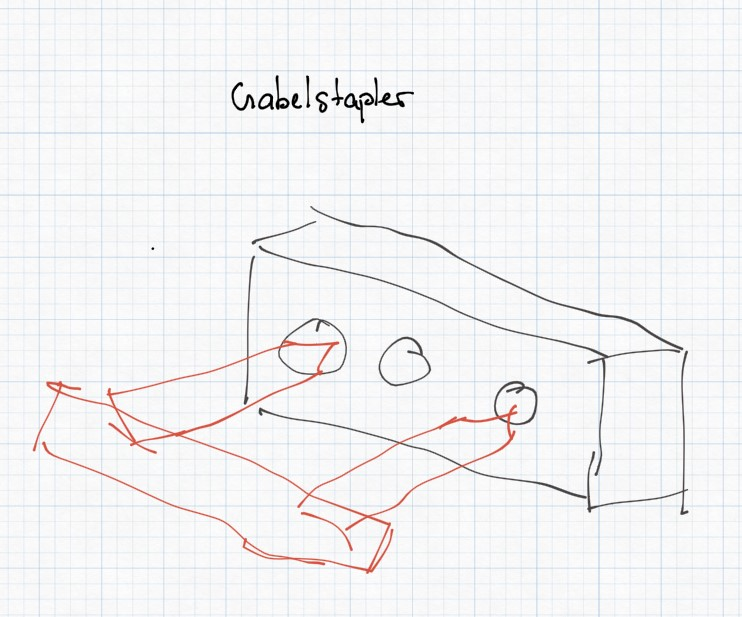
\includegraphics[width=0.48\textwidth]{img/technologierecherche/Aufnahme/Gabelstapler.jpg}
        \caption{Prinzip angelehnt an einen Gabelstapler}
        \label{img:tech_Gaplerstapler}
\end{figure}

\begin{minipage}[t]{0.48\textwidth}
    \begin{items}
          \item [Vorteile]
          \item Einfache Griffkonstruktion
          \item Sehr guter Halt des Hindernisses Richtung Boden
    \end{items}
\end{minipage}
\hfill
\begin{minipage}[t]{0.48\textwidth}
    \begin{items}
          \item [Nachteile]
          \item Schwierigere Arm Konstruktion für Präzision
          \item Hohe Präzision bei Sensoren erforderlich
          \item Löcher müssen erkannt werden
          \item Kann in Richtung Fahrrichtung herausfallen, Vorkehrung muss getroffen werden
    \end{items}
\end{minipage}
\newpage
%%%%%-----------------------------------------------
\paragraph{Vakuumgreifer}
Benutzt Unterdruck, um das Hindernis zu "greifen".

\begin{figure}[h!]
        \centering
        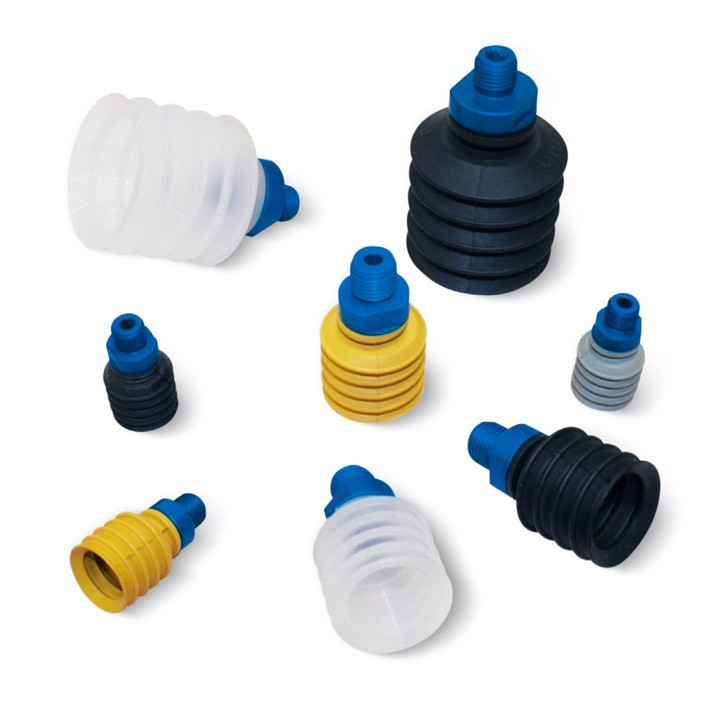
\includegraphics[width=0.48\textwidth]{img/technologierecherche/Aufnahme/Vakuumgreifer.jpg}
        \caption[Aufnahme über Vakuumgreifer]{Aufnahme über Vakuumgreifer \footnotemark}
        \label{img:tech_Vakuumgreifer}
\end{figure}
\footnotetext{Quelle: \url{https://www.youtube.com/shorts/alxwWgzSVss}}

\begin{minipage}[t]{0.48\textwidth}
    \begin{items}
          \item [Vorteile]
          \item Aussergewöhnliche Art, das Hindernis zu greifen
    \end{items}
\end{minipage}
\hfill
\begin{minipage}[t]{0.48\textwidth}
    \begin{items}
          \item [Nachteile]
          \item Darf nicht in die Löcher fallen → muss verhindert werden
          \item Unklar, ob Greifkraft reicht
          \item Benötigt weiteren Motor an Bord
    \end{items}
\end{minipage}
\newpage
%%%%%-----------------------------------------------
\paragraph{Klemmen Längsweg}
Klemmt über Längsweg das Hindernis, um dadurch einen sicheren Halt zu generieren.

\begin{figure}[h!]
        \centering
        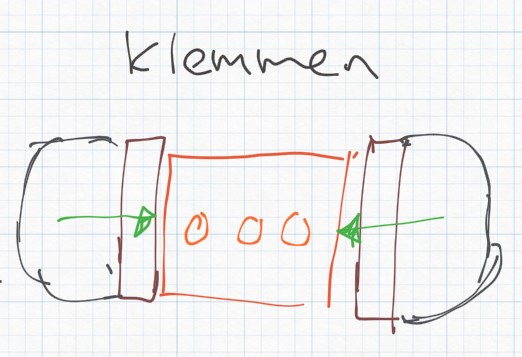
\includegraphics[width=0.48\textwidth]{img/technologierecherche/Aufnahme/Laengsweg_Griff.jpg}
        \caption{Klemme über Längsweg des Hindernisses}
        \label{img:tech_Laengsweg_Griff}
\end{figure}

\begin{minipage}[t]{0.48\textwidth}
    \begin{items}
          \item [Vorteile]
          \item Wenig Präzision vom Arm erforderlich (Wenn überhaupt arm erforderlich)
          \item Sicherer halt
    \end{items}
\end{minipage}
\hfill
\begin{minipage}[t]{0.48\textwidth}
    \begin{items}
          \item [Nachteile]
          \item Damit Arm wegfällt müsste ein Mechanismus zum Anheben gemacht werden (Damit Regelkonform)
          \item Die Konstruktion eines Armes würde hier komplexer ausfallen 
    \end{items}
\end{minipage}
\newpage
%%%%%-----------------------------------------------
\paragraph{Klemmen Breitenweg}
Klemme über Breitenweg des Hindernisses. Dieses Prinzip kann sogar modifiziert
werden, um Berührungssensoren zu verwenden

\begin{figure}[h]
        \centering
        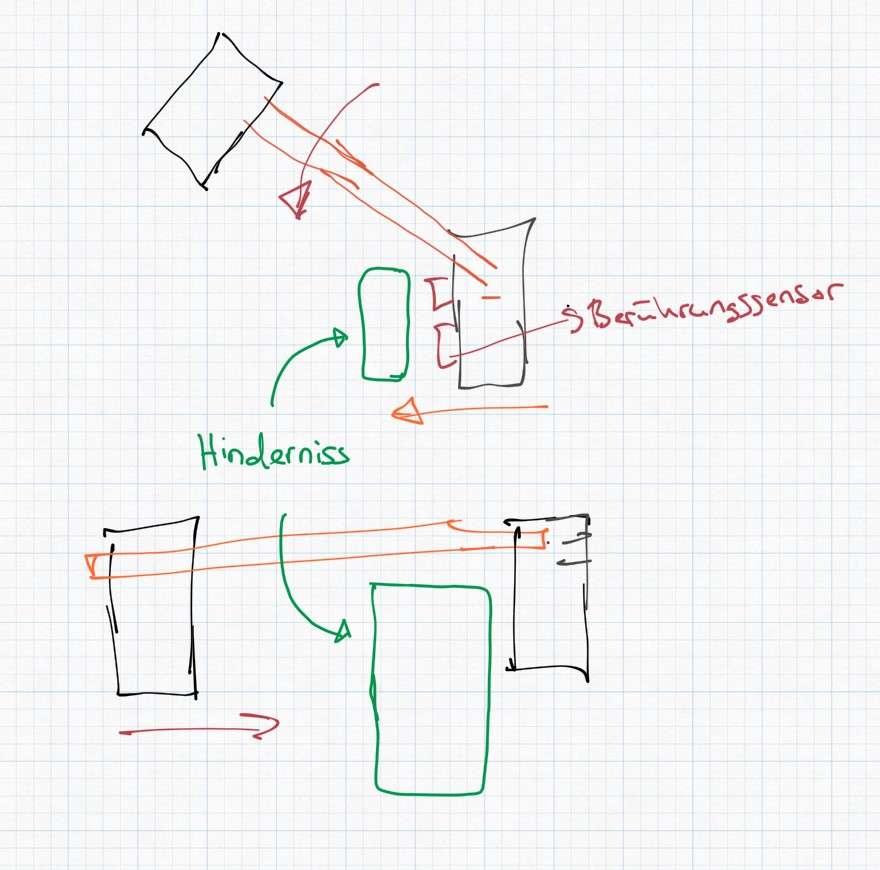
\includegraphics[width=0.48\textwidth]{img/technologierecherche/Aufnahme/Breiterweg_Griff.jpg}
        \caption{Klemme über Breitenweg des Hindernisses}
        \label{img:tech_Breiterweg_Griff}
\end{figure}

\begin{minipage}[t]{0.48\textwidth}
    \begin{items}
          \item [Vorteile]
          \item Wenig Präzision vom Arm erforderlich (Wenn überhaupt arm erforderlich)
          \item Sensoren können im Griff verbaut werden (Berührungssensoren)
          \item Sicherer halt
    \end{items}
\end{minipage}
\hfill
\begin{minipage}[t]{0.48\textwidth}
    \begin{items}
          \item [Nachteile]
          \item Damit Arm wegfällt, müsste eine komplexere Greifvorrichtung gemacht werden
          \item Damit Arm wegfällt, müsste ein Mechanismus zum Anheben gemacht werden (Damit Regelkonform)
    \end{items}
\end{minipage}
\newpage
%%%%%-----------------------------------------------
\paragraph{Mantis (mit elastischen Klemmen)}
Es wird über Längsweg gegriffen, es wird ausgenutzt das es auf den Seiten Verbindungen zum Zusammenstecken der Hindernisse hat, dadurch können auch elastische Materialien verwendet werden zum greifen.

\begin{figure}[h!]
        \centering
        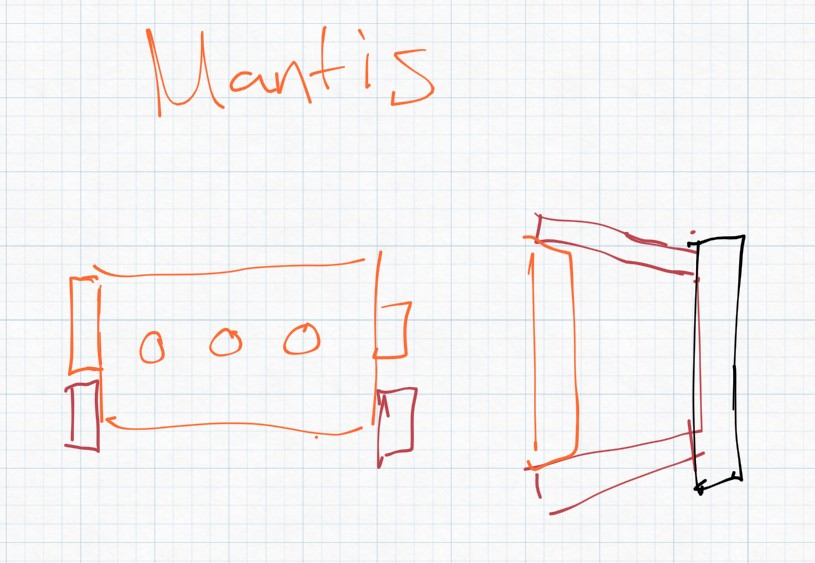
\includegraphics[width=0.48\textwidth]{img/technologierecherche/Aufnahme/Mantis.jpg}
        \caption{Mantis Skizze}
        \label{img:tech_Mantis}
\end{figure}

\begin{minipage}[t]{0.48\textwidth}
    \begin{items}
          \item [Vorteile]
          \item Wenig Präzision vom Arm erforderlich (Wenn überhaupt arm erforderlich).
          \item Weniger Präzision von Sensoren erforderlich (Ausgleich durch Elastizität).
    \end{items}
\end{minipage}
\hfill
\begin{minipage}[t]{0.48\textwidth}
    \begin{items}
          \item [Nachteile]
          \item Das Hindernis könnte davon geschleudert werden.
          \item Könnte Probleme bereiten, dass die Klemmen nicht auf gleicher Höhe ansetzten.
    \end{items}
\end{minipage}
\newpage

\paragraph{Bagger}
Die Konstruktion ist an einen Bagger angelegt und wurde im vorraus schon zum Teil recherchiert.

\begin{figure}[h!]
        \centering
        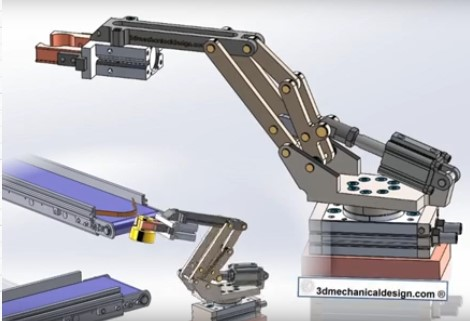
\includegraphics[width=0.48\textwidth]{img/technologierecherche/Rotation/kran.jpg}
        \caption[Bagger änhliche Konstruktion]{Bagger ähnliche Konstruktion \footnotemark} 
        \label{img:tech_kran}
\end{figure}
\footnotetext{Quelle: \url{https://www.youtube.com/watch?v=VZRFHJfUkq4}}

\begin{minipage}[t]{0.48\textwidth}
    \begin{items}
          \item [Vorteile]
          \item Sehr gut ansteuerbar
          \item Kann mit viel Greifmethoden gebrauch werden
          \item Beispiel vorhanden
          \item Sensoren auf Gefährt möglich
    \end{items}
\end{minipage}
\hfill
\begin{minipage}[t]{0.48\textwidth}
    \begin{items}
          \item [Nachteile]
          \item Komplexer Aufbau
    \end{items}
\end{minipage}
\newpage
%%--------------------------------------------------------
\paragraph{Rotation Fahrzeug}
Anstatt einen Arm wo sich dreht, dreht sich das ganze Fahrzeug mit dem Hindernis

\begin{figure}[h!]
        \centering
        \includegraphics[width=0.48\textwidth]{img/technologierecherche/Rotation/seitlich_mit_räder.jpg}
        \caption{Für die Rotation wird das ganze Fahrzeug gewendet}
        \label{img:tech_seitlich_mit_räder}
\end{figure}

\begin{minipage}[t]{0.48\textwidth}
    \begin{items}
          \item [Vorteile]
          \item Kann mit vielen Greifmethoden gebraucht werden
          \item Sehr einfach
          \item Sensoren auf Gefährt möglich
    \end{items}
\end{minipage}
\hfill
\begin{minipage}[t]{0.48\textwidth}
    \begin{items}
          \item [Nachteile]
          \item Präzision hängt von Fahrzeug Positionssensoren ab
          \item Steuerbarkeit kommt auf die Manövrierfähigkeit des Fahrzeuges an 
    \end{items}
\end{minipage}
\newpage
%%--------------------------------------------------------
\paragraph{Kran}
Diese Konstruktion ist an einen Kran angelegt und Greift das Objekt von oben herab. Ein Beispiel wurde vorab schon recherchiert.

\begin{figure}[H]
        \centering
        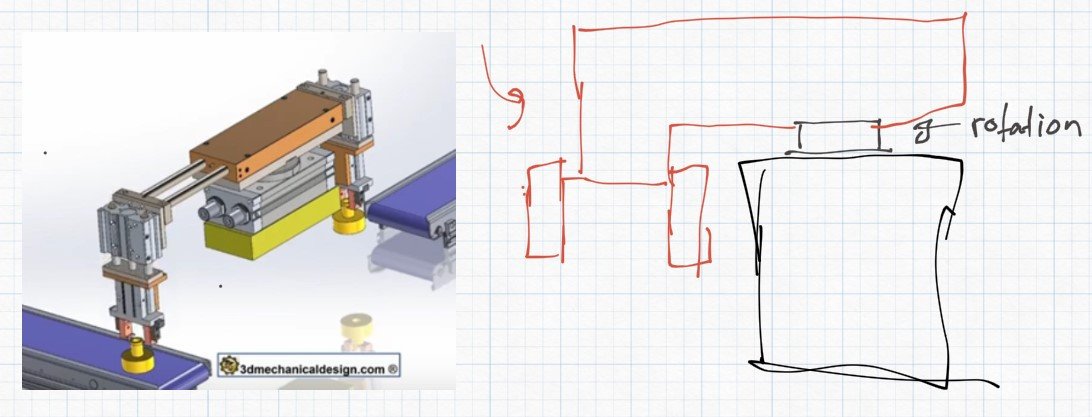
\includegraphics[width=0.48\textwidth]{img/technologierecherche/Rotation/seitlich_mit_rotation.jpg}
        \caption[Konstruktion an einen Kran angelegt]{Konstruktion an einen Kran angelegt \footnotemark} 
        \label{img:tech_seitlich_mit_rotation}
\end{figure}
\footnotetext{Quelle: \url{https://www.youtube.com/watch?v=J7LGSNhFTU4}}

\begin{minipage}[t]{0.48\textwidth}
    \begin{items}
          \item [Vorteile]
          \item Beispiel vorhanden
          \item Sensoren auf Gefährt möglich
    \end{items}
\end{minipage}
\hfill
\begin{minipage}[t]{0.48\textwidth}
    \begin{items}
          \item [Nachteile]
          \item Komplexer Aufbau, wenn Arm kleine Korrekturen vornehmen soll
          \item Präzision hängt ansonsten von Fahrzeug Manövrierfähigkeit ab
    \end{items}
\end{minipage}
\newpage
%%--------------------------------------------------------
\paragraph{Lagerung am Ende Arm}
Damit das Hindernis wieder aufrecht steht, wird die Rotation am Arm selber durchgeführt. 

\begin{figure}[H]
        \centering
        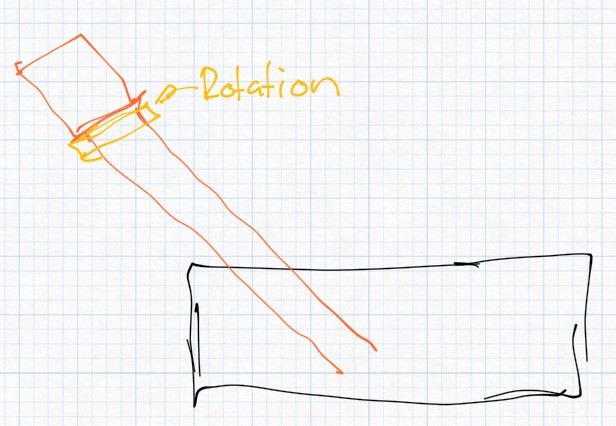
\includegraphics[width=0.48\textwidth]{img/technologierecherche/Rotation/ueberkopf_griff_gelagert.jpg}
        \caption{Skizze Rotation am Arm}
        \label{img:tech_ueberkopf_griff_gelagert}
\end{figure}

\begin{minipage}[t]{0.48\textwidth}
    \begin{items}
          \item [Vorteile]
          \item Durch fixe Armlänge kann Präzision gewährleistet werden
    \end{items}
\end{minipage}
\hfill
\begin{minipage}[t]{0.48\textwidth}
    \begin{items}
          \item [Nachteile]
          \item Geht über Kopf und dadurch ist die Platzierung der Sensoren eingeschränkt.
          \item Umsetzung der Technologie unklar
          \item Unklar wie viele Greifmethoden verwendet werden können bei einer solchen Rotation
    \end{items}
\end{minipage}
\newpage
%%--------------------------------------------------------
\paragraph{Lagerung am Hindernis}
Damit das Hindernis wieder aufrecht steht, wird die Rotation bei dem Griff selber durchgeführt.

\begin{figure}[H]
        \centering
        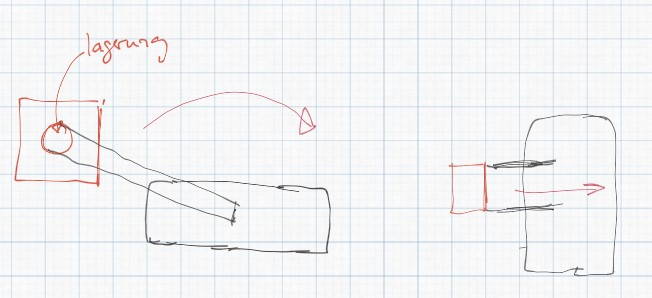
\includegraphics[width=0.48\textwidth]{img/technologierecherche/Rotation/ueberkopf_objekt_gelagert.jpg}
        \caption{Skizze Lagerung am Hindernis} 
        \label{img:tech_ueberkopf_objekt_gelagert}
\end{figure}

\begin{minipage}[t]{0.48\textwidth}
    \begin{items}
          \item [Vorteile]
          \item Elegante Lösung um das aufrecht Stehen des Hindernisses zu gewährleisten.
          \item Können viel Greifmethoden verwendet werden
    \end{items}
\end{minipage}
\hfill
\begin{minipage}[t]{0.48\textwidth}
    \begin{items}
          \item [Nachteile]
          \item Geht über Kopf dadurch Sensoren, Platzierung eingeschränkt
          \item Je nach Greifmethode kann diese Art an Komplexität gewinnen
    \end{items}
\end{minipage}
\newpage
%%--------------------------------------------------------
\paragraph{Greifhacken}
Eine Greifhacken artige Konstruktion, die die Löcher des Hindernisses ausnutzt

\begin{figure}[h!]
        \centering
        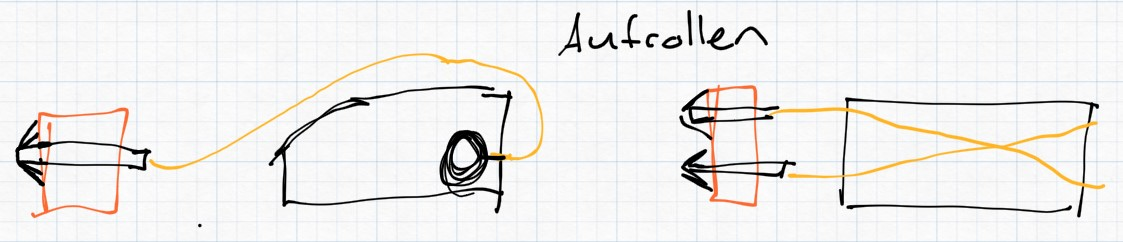
\includegraphics[width=0.48\textwidth]{img/technologierecherche/Rotation/harponne.jpg}
        \caption{Eine Greifhacken artige Konstruktion}
        \label{img:tech_harponne}
\end{figure}

\begin{minipage}[t]{0.48\textwidth}
    \begin{items}
          \item [Vorteile]
          \item Sehr einzigartige Methode
    \end{items}
\end{minipage}
\hfill
\begin{minipage}[t]{0.48\textwidth}
    \begin{items}
          \item [Nachteile]
          \item Muss Gabelstapler als Aufnahme verwendet werden
          \item Sehr unklar, ob funktioniert
          \item Motor muss stark genug sein, Hindernis zu ziehen
          \item Gehäuse muss genug robust sein → Das Hindernis wird über das Gehäuse gezogen
          \item Geht über Kopf → dadurch Sensoren Platzierung eingeschränkt
    \end{items}
\end{minipage}
\newpage
%%--------------------------------------------------------
\subsection{Antrieb und Orientierung}
Im folgenden Abschnitt werden die einzelnen elektrischen Varianten verglichen. Indem zu jeder Variante die Vor- und Nachteile aufgelistet werden. Dies vereinfacht später, beim morphologischen Kasten, die möglichen Lösungswege.

\subsubsection{Antrieb}

In diesem Teil werden die verschiedenen elektrische Antriebe aufgelistet. 

\paragraph{DC-Motor}

Der DC-Motor ist ein Gleichstrom-Motor, der mit Bürsten am Kommutator arbeitet. 

\begin{minipage}[t]{0.48\textwidth}
\begin{items}
  \item [Vorteile]
  \item Einfache Drehzahlsteuerung
  \item Hohe Drehzahlen
  \item Hohes Drehmoment
\end{items}
\end{minipage}
\hfill
\begin{minipage}[t]{0.48\textwidth}
\begin{items}
  \item [Nachteile]
  \item EMV Störung durch Funkenbildung
  \item Schlechte Wärmeabführung
\end{items}
\end{minipage}

\paragraph{Brushless DC-Motor}

Brushless DC Motoren(BLDC) werden häufig im Modellbau oder Drohnen eingesetzt. Diese haben gegnüber normalen DC-Motoren keine Bürsten. Sie besitzen drei Wicklungen auf dem Stator und haben Im Rotor einen permanent Magneten. Die Spulen werden nun so angesteuert, dass es ein wechselndes Magnetfeld gibt. Dieses Drehfeld bringt den Rotor zur Drehung. 

\begin{minipage}[t]{0.48\textwidth}
\begin{items}
  \item [Vorteile]
  \item Hohe Effizienz
  \item Präzise Ansteuerung
  \item Hohe Lebensdauer
\end{items}
\end{minipage}
\hfill
\begin{minipage}[t]{0.48\textwidth}
\begin{items}
  \item [Nachteile]
  \item Komplexe Ansteuerung
  \item Hohe Kosten
\end{items}
\end{minipage}


\paragraph{Schrittmotor}

Der Schrittmotor wird vor allem bei genauen Positioniersystem wie Roboter, CNC oder auch 3D-Drucker eingesetzt. Diese Motoren haben viel mehr Wicklungen als ein BLDC. Dadurch können Sie kleinere Winkel anfahren und sind somit präzise Positionierungsantriebe. 

\begin{minipage}[t]{0.48\textwidth}
\begin{items}
  \item [Vorteile]
  \item Präzise Ansteuerung
  \item Hohe Drehmoment bei tiefen Drehzahlen
  \item Kein Encoder nötig (bei genügender Auslegung)
\end{items}
\end{minipage}
\hfill
\begin{minipage}[t]{0.48\textwidth}
\begin{items}
  \item [Nachteile]
  \item Reduzierte Leistung hoher bei Geschwindigkeit
  \item Hoher Stromverbrauch
  \item Erzeugen Vibrationen bei hohen Drehzahlen
\end{items}
\end{minipage}

\subsubsection{Orientierung / Sensorik}

Es wird darauf eingegangen, wie das Fahrzeug seine Umgebung wahrnehmen kann. Dabei werden wieder die einzelnen Vor- und Nachteile aufgelistet.

\paragraph{Linienfolger}
Ein Liniensensor funktioniert mit mehreren Fotodioden und LEDs. Die LEDs beleuchten den Boden und die in einer Reihe angeordneten Fotodioden nehmen mehr oder weniger von diesem reflektiertem Licht auf. Je nach Untergrund wird es mehr oder weniger reflektiert. So kann man die Linie erkennen und dieser folgen.
 

\begin{minipage}[t]{0.48\textwidth}
\begin{items}
  \item [Vorteile]
  \item schnelle Reaktion
  \item einfacher Aufbau
\end{items}
\end{minipage}
\hfill
\begin{minipage}[t]{0.48\textwidth}
\begin{items}
  \item [Nachteile]
  \item Hoher Kontrast nötig
  \item Störungsanfällig auf Fremdlicht
  \item Kalibrierung notwendig
\end{items}
\end{minipage}

\paragraph{Infrarot}
Mit Infrarot (IR) Sensoren können Objekte erkannt werden und ebenso die Distanz zu Ihnen ermittelt werden.

\begin{minipage}[t]{0.48\textwidth}
\begin{items}
  \item [Vorteile]
  \item Schnelle Reaktionszeit
  \item Hohe Empfindlichkeit
  \item Robust und langlebig
\end{items}
\end{minipage}
\hfill
\begin{minipage}[t]{0.48\textwidth}
\begin{items}
  \item [Nachteile]
  \item Begrenzte Reichweite
  \item Abhängigkeit Oberflächenbeschaffenheit
  \item Störungen durch andere IR-Quellen
\end{items}
\end{minipage}

\paragraph{Ultraschall}
Ein Ultraschallsensor sendet Schallwellen aus und kann mit deren Reflexion von Objekten, diese erkennen und die Distanz zu Ihnen ermitteln.

\begin{minipage}[t]{0.48\textwidth}
\begin{items}
  \item [Vorteile]
  \item Material unabhängig
  \item Hohe Präzision
  \item Robust gegenüber Umwelteinflüssen
\end{items}
\end{minipage}
\hfill
\begin{minipage}[t]{0.48\textwidth}
\begin{items}
  \item [Nachteile]
  \item Tote Zone in der Nähe des Sensors
  \item Unpräzise bei komplexer Umgebung
  \item Kleine Objekte schwer zu detektieren
\end{items}
\end{minipage}

\paragraph{Encoder}
Ein Encoder detektiert die Umdrehungen eines Motors und wandelt dies in ein digitales Signal um. Mit diesem Signal kann die Steuerung den Motor präzise ansteuern.
 

\begin{minipage}[t]{0.48\textwidth}
\begin{items}
  \item [Vorteile]
  \item Hohe Präzision
  \item Schnelle Reaktionszeit
\end{items}
\end{minipage}
\hfill
\begin{minipage}[t]{0.48\textwidth}
\begin{items}
  \item [Nachteile]
  \item Hohe Kosten
  \item Anfällig durch Schmutz oder EMV
\end{items}
\end{minipage}


\subsubsection{Energiequelle}

Im unteren Teil werden die verschiedenen Energiequellen untersucht.

\paragraph{Lithium-Polymer}
Der Lithium-Polymer (LiPo) Akku ist ein formbarer Akku, der vor allem im Modellbau und bei Drohnen eingesetzt wird.
 

\begin{minipage}[t]{0.48\textwidth}
\begin{items}
  \item [Vorteile]
  \item Leicht und flexibel in der Formgebung
  \item Hohe Leistungsdichte
  \item Hohe Entladerate
\end{items}
\end{minipage}
\hfill
\begin{minipage}[t]{0.48\textwidth}
\begin{items}
  \item [Nachteile]
  \item Empfindlichkeit zu Über- und Tiefenentladung
  \item Empfindlich auf mechanische Schläge
  \item Sicherheit Feuergefahr
\end{items}
\end{minipage}


\paragraph{Lithium-Ionen}

Der Lithium-Ionen (Li-Ion) Akku ist ein robuster Akku der in Laptop und Smartphones eingesetzt wird. Da dieser kein Memory Effekt besitzt. Der Memory Effekt beschreibt, wenn der Akku nicht ganz entladen wurde und dann wieder aufgeladen wird, das er diesen Punkt als tiefesten Zustand "merkt".

\begin{minipage}[t]{0.48\textwidth}
\begin{items}
  \item [Vorteile]
  \item Lange Lebensdauer
  \item Hohe Energiedichte
  \item Kein Memory-Effekt
\end{items}
\end{minipage}
\hfill
\begin{minipage}[t]{0.48\textwidth}
\begin{items}
  \item [Nachteile]
  \item Temperaturempfindlich
  \item Hohe Kosten
  \item Sicherheit Feuergefahr
\end{items}
\end{minipage}
 

\paragraph{Nickel-Metallhydrid}

Nickel-Metallhydrid (NiMH) Akkus sind in vielen Haushaltsgeräten, Digitalkameras oder Taschenlampen zu finden. 

\begin{minipage}[t]{0.48\textwidth}
\begin{items}
  \item [Vorteile]
  \item Moderate Energiedichte
  \item Geringer Memory Effekt
  \item Sicher
\end{items}
\end{minipage}
\hfill
\begin{minipage}[t]{0.48\textwidth}
\begin{items}
  \item [Nachteile]
  \item Selbstentladung
  \item Kapazitätsverlust
  \item Temperaturempfindlich
\end{items}
\end{minipage}

\end{document}